%%%%%%%%%%%%%%%%%%%%%%%%%%%%%%%%%%%%%%%%%
% Wenneker Article
% LaTeX Template
% Version 2.0 (28/2/17)
%
% This template was downloaded from:
% http://www.LaTeXTemplates.com
%
% Authors:
% Vel (vel@LaTeXTemplates.com)
% Frits Wenneker
%
% License:
% CC BY-NC-SA 3.0 (http://creativecommons.org/licenses/by-nc-sa/3.0/)
%
%%%%%%%%%%%%%%%%%%%%%%%%%%%%%%%%%%%%%%%%%

%----------------------------------------------------------------------------------------
%	PACKAGES AND OTHER DOCUMENT CONFIGURATIONS
%----------------------------------------------------------------------------------------

\documentclass[12pt, a4paper, twocolumn]{article} % 10pt font size (11 and 12 also possible), A4 paper (letterpaper for US letter) and two column layout (remove for one column)

%%%%%%%%%%%%%%%%%%%%%%%%%%%%%%%%%%%%%%%%%
% Wenneker Article
% Structure Specification File
% Version 1.0 (28/2/17)
%
% This file originates from:
% http://www.LaTeXTemplates.com
%
% Authors:
% Frits Wenneker
% Vel (vel@LaTeXTemplates.com)
%
% License:
% CC BY-NC-SA 3.0 (http://creativecommons.org/licenses/by-nc-sa/3.0/)
%
%%%%%%%%%%%%%%%%%%%%%%%%%%%%%%%%%%%%%%%%%

%----------------------------------------------------------------------------------------
%	PACKAGES AND OTHER DOCUMENT CONFIGURATIONS
%----------------------------------------------------------------------------------------

\usepackage[english]{babel} % English language hyphenation

\usepackage{microtype} % Better typography

\usepackage{amsmath,amsfonts,amsthm} % Math packages for equations

\usepackage[svgnames]{xcolor} % Enabling colors by their 'svgnames'

\usepackage[hang, small, labelfont=bf, up, textfont=it]{caption} % Custom captions under/above tables and figures

\usepackage{booktabs} % Horizontal rules in tables

\usepackage{lastpage} % Used to determine the number of pages in the document (for "Page X of Total")

\usepackage{graphicx} % Required for adding images

\usepackage{enumitem} % Required for customising lists
\setlist{noitemsep} % Remove spacing between bullet/numbered list elements

\usepackage{sectsty} % Enables custom section titles
\allsectionsfont{\usefont{OT1}{phv}{b}{n}} % Change the font of all section commands (Helvetica)

%----------------------------------------------------------------------------------------
%	MARGINS AND SPACING
%----------------------------------------------------------------------------------------

\usepackage{geometry} % Required for adjusting page dimensions

\geometry{
	top=1cm, % Top margin
	bottom=1.5cm, % Bottom margin
	left=2cm, % Left margin
	right=2cm, % Right margin
	includehead, % Include space for a header
	includefoot, % Include space for a footer
	%showframe, % Uncomment to show how the type block is set on the page
}

\setlength{\columnsep}{7mm} % Column separation width

%----------------------------------------------------------------------------------------
%	FONTS
%----------------------------------------------------------------------------------------

\usepackage[T1]{fontenc} % Output font encoding for international characters
\usepackage[utf8]{inputenc} % Required for inputting international characters

\usepackage{XCharter} % Use the XCharter font

%----------------------------------------------------------------------------------------
%	HEADERS AND FOOTERS
%----------------------------------------------------------------------------------------

\usepackage{fancyhdr} % Needed to define custom headers/footers
\pagestyle{fancy} % Enables the custom headers/footers

\renewcommand{\headrulewidth}{0.0pt} % No header rule
\renewcommand{\footrulewidth}{0.4pt} % Thin footer rule

\renewcommand{\sectionmark}[1]{\markboth{#1}{}} % Removes the section number from the header when \leftmark is used

%\nouppercase\leftmark % Add this to one of the lines below if you want a section title in the header/footer

% Headers
\lhead{} % Left header
\chead{\textit{\thetitle}} % Center header - currently printing the article title
\rhead{} % Right header

% Footers
\lfoot{} % Left footer
\cfoot{} % Center footer
\rfoot{\footnotesize Page \thepage\ of \pageref{LastPage}} % Right footer, "Page 1 of 2"

\fancypagestyle{firstpage}{ % Page style for the first page with the title
	\fancyhf{}
	\renewcommand{\footrulewidth}{0pt} % Suppress footer rule
}

%----------------------------------------------------------------------------------------
%	TITLE SECTION
%----------------------------------------------------------------------------------------

\newcommand{\authorstyle}[1]{{\large\usefont{OT1}{phv}{b}{n}\color{DarkRed}#1}} % Authors style (Helvetica)

\newcommand{\institution}[1]{{\footnotesize\usefont{OT1}{phv}{m}{sl}\color{Black}#1}} % Institutions style (Helvetica)

\usepackage{titling} % Allows custom title configuration

\newcommand{\HorRule}{\color{DarkGoldenrod}\rule{\linewidth}{1pt}} % Defines the gold horizontal rule around the title

\pretitle{
	\vspace{-30pt} % Move the entire title section up
	\HorRule\vspace{10pt} % Horizontal rule before the title
	\fontsize{32}{36}\usefont{OT1}{phv}{b}{n}\selectfont % Helvetica
	\color{DarkRed} % Text colour for the title and author(s)
}

\posttitle{\par\vskip 15pt} % Whitespace under the title

\preauthor{} % Anything that will appear before \author is printed

\postauthor{ % Anything that will appear after \author is printed
	\vspace{10pt} % Space before the rule
	\par\HorRule % Horizontal rule after the title
	\vspace{20pt} % Space after the title section
}

%----------------------------------------------------------------------------------------
%	ABSTRACT
%----------------------------------------------------------------------------------------

\usepackage{lettrine} % Package to accentuate the first letter of the text (lettrine)
\usepackage{fix-cm}	% Fixes the height of the lettrine

\newcommand{\initial}[1]{ % Defines the command and style for the lettrine
	\lettrine[lines=3,findent=4pt,nindent=0pt]{% Lettrine takes up 3 lines, the text to the right of it is indented 4pt and further indenting of lines 2+ is stopped
		\color{DarkGoldenrod}% Lettrine colour
		{#1}% The letter
	}{}%
}

\usepackage{xstring} % Required for string manipulation

\newcommand{\lettrineabstract}[1]{
	\StrLeft{#1}{1}[\firstletter] % Capture the first letter of the abstract for the lettrine
	\initial{\firstletter}\textbf{\StrGobbleLeft{#1}{1}} % Print the abstract with the first letter as a lettrine and the rest in bold
}

%----------------------------------------------------------------------------------------
%	BIBLIOGRAPHY
%----------------------------------------------------------------------------------------

\usepackage[backend=bibtex,style=authoryear,natbib=true]{biblatex} % Use the bibtex backend with the authoryear citation style (which resembles APA)

\addbibresource{bibliography.bib} % The filename of the bibliography

\usepackage[autostyle=true]{csquotes} % Required to generate language-dependent quotes in the bibliography
 % Specifies the document structure and loads requires packages

%----------------------------------------------------------------------------------------
%	ARTICLE INFORMATION
%----------------------------------------------------------------------------------------

\title{Microservicii: șabloane, performanță, evoluție} % The article title

\author{
	\authorstyle{Sergiu Breban\textsuperscript{1}} % Authors
	\newline\newline % Space before institutions
	\textsuperscript{1}\institution{Universitatea Babeș-Bolyai, Cluj-Napoca, Cluj}\\ % Institution 1
}

% Example of a one line author/institution relationship
%\author{\newauthor{John Marston} \newinstitution{Universidad Nacional Autónoma de México, Mexico City, Mexico}}

\date{\today} % Add a date here if you would like one to appear underneath the title block, use \today for the current date, leave empty for no date

%----------------------------------------------------------------------------------------

\begin{document}

\maketitle % Print the title

\thispagestyle{firstpage} % Apply the page style for the first page (no headers and footers)

%----------------------------------------------------------------------------------------
%	ABSTRACT
%----------------------------------------------------------------------------------------

\abstract{Arhitectura bazată pe microservicii este inspirată de tehnicile de calcul orientate pe servicii care au câștigat popularitate în ultima perioadă și este folosită pentru a construi sisteme complexe compuse din procese mici, independente și decuplate. Vom prezenta principalele caracteristici ale acestei tehnici, cu avantaje și dezavantaje, inclusiv impactul acestei abordări asupra performanței rețelei de comunicare, dar și câteva etape din dezvoltarea acestei arhitecturi.}

%----------------------------------------------------------------------------------------
%	ARTICLE CONTENTS
%----------------------------------------------------------------------------------------

\section{Introducere}

Abordarea arhitecturală bazată pe microservicii este relativ recentă în cadrul modelelor folosite în industria software. Această abordare folosește un set de servicii independente, de mărime cât mai mică, cu roluri bine determinate în cadrul domeniului, fiecare rulând în cadrul propriului process. Aceste servicii comunică în general prin mecanisme contruite în jurul protocolului HTTP.\citep{uckelmann2011architectural} Astfel de servicii pot fi instalate și lansate independent. În ultimii ani, odată cu apariția cloud computing-ului, microserviciile au câștigat popularitate, acest șablon arhitectural fiind cel mai potrivit pentru a profita de avantajele oferite de cloud, printre care disponibilitatea și scalabilitatea. Acest lucru poate fi realizat prin folosirea de virtualizarea bazată pe containere, care oferă o alternativă mai bună la hypervizori\citep{soltesz2007container}, prin implementări de tipul Docker, care folosește containere bazate pe sistemul de operare Linux. Modelul opus celui bazat pe microservicii este modelul monolitic, care conține întreaga logică a sistemului într-o singură unitate instalabilă.\citep{richardson2014pattern} Această abordare nu mai este potrivită după ce dimensiunea sistemului crește. Un sistem monolitic este mai greu de întreținut și modificat, oferă o scalabilitate limitată și limitează alegerea tehnologiilor pentru dezvoltatori.\citep{dragoni2017microservices}

\clearpage

\section{Șabloane} Dar arhitectura bazată pe micorservicii are și dezavantaje, cel mai mare fiind creat de complexitatea necesară pentru a crea un astfel de sistem distribuit și toate elementele necesare, de la comunicarea între servicii și procesarea transacțională. De asemenea, va crește și complexitatea instalării, fiind nevoie de gestiunea mai multor tipuri de servicii, dar și consumul de memorie în cadrul sistemelor folosite, datorită spațiului de adrese necesar fiecărui serviciu. Pentru a împărți un sistem monolitic în mai multe servicii independente este nevoie de diferite abordări, un tipar fiind delimitarea acestora pe baza cazurilor de utilizare. O altă abordare pentru partiționare este folosirea verbelor, a numelor sau a resurselor pentru delimitare, fiecare serviciu fiind responsabil pentru o anumită operație sau mai multe operații pe anumite entități.\citep{hassan2010provisioning} Se ține cont de pricipiul responsabilității unice (Single Responsible Principle (SRP)) pentru a garanta că fiecare serviciu are doar un set mic, bine definit, de responsabilități.\par
Microserviciile pot fi văzut ca niște componente software, unități software care unde înlocuibile independent, și au nevoie de un anumite tip ce proceduri chemate la distanță pentru comunicare. Pentru a garanta succesul unei astfel de arhitecturi, este nevoie de o interfață de comunicare atent construită și care poate fi ușor întreținută. Câteva primitive necesare pentru a asigura aceasta sunt: apeluri de tip cerere/răspuns cu date structura arbitrare, procesarea de eventimente asincrone în timp real în ambele direcții de comunicare, folosirea unui serviciu de serializare a mesajelor de tipul JSON, XML.\par
Componenta de rețea este foarte importantă în cadrul oricărei arhitecturi distribuite, deoarece oferă comunicare între diversele servicii. În cadrul arhitecuturii bazate pe microservicii, mai multe scenarii de comunicare sunt posibile. Un prim scenariu este cel în care aplicația client folosește fiecare serviciu în mod direct.

\begin{figure}[h]
\caption{Apeluri directe}
\centering
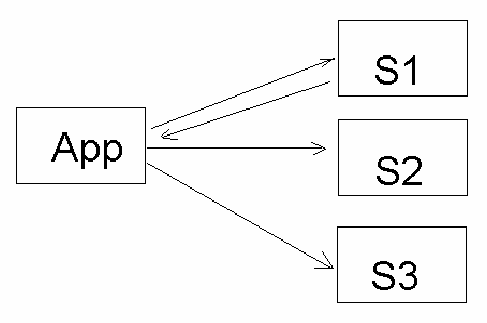
\includegraphics[width=0.4\textwidth]{direct}
\end{figure}

Acesta este cel mai flexibil mod. Pentru a scădea numărul de apeluri la distanță, se pot folosi diverse modele de caching sau middleware, ca și în figura de mai jos.

\begin{figure}[h]
\caption{Un gateway pentru microservicii}
\centering
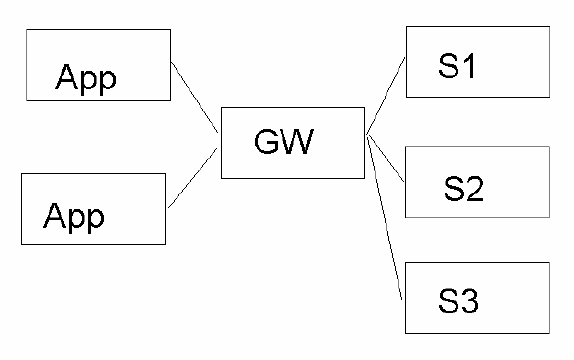
\includegraphics[width=0.4\textwidth]{gateway}
\end{figure}

Al treilea șablon folosit în gestionarea arhitectucrii cu microservicii este bazat pe un service bus, care permite aplicațiilor să trimită cereri și să citească răspunsurile mai târziu. Acest model facilitează adăugarea de noi componente fără modificarea celor existente.

\begin{figure}[h]
\caption{Service bus}
\centering
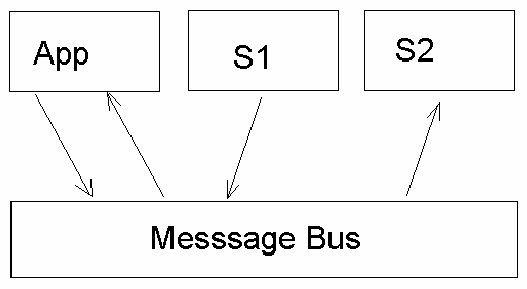
\includegraphics[width=0.4\textwidth]{bus}
\end{figure}

\clearpage

\section{Perfomanțe} Virtualizarea bazată pe containere este văzută ca o soluție mai scalabilă și performantă decât hypervizorii în implementarea sistemelor bazate pe microservicii, dar aceasta din urmă este implementată cel mai des în sistemele de cloud computing. \citep{felter2015updated} oferă o analiză detaliată a consumului de memorie, CPU, stocare și resurse de rețea pentru a compara instalările tradiționale bazate pe mașini virtuale și utilizarea de containere Linux oferite de Docker, ajungând la concluzia că aceastea oferă aporximativ aceeași performanță în diferite procesări, fără a analiza însă impactul containerelor deasupra hypervizorilor.\par Este nevoie de analiza performanței rețelei de comunicare a containerelor, a rețelelor virtuale definite în cadrul sistemelor software și a nivelelor de criptare asupra sistemelor distribuite bazate pe cloud care folosesc protocoale bazate pe HTTP și REST. Pentru a măsura acestea s-au făcut mai multe experimente, cel de referință fiind folosit pentru comparare. Sistemul de referință a fost un sistem bazat pe microservicii, instalat pe mai multe mașini virtuale și folosind REST și HTTP pentru comunicare. Performanțele acestui sistem au fost comparate pe rând cu adăugarea de containere, creare unei rețele virtuale definite software și aduăgarea unui nivel de criptare, pentru a măsura impactul fiecărei modificări. Se măsoară rata de transfer a mesajelor de mărime m (bytes), notate trans(m). Experimentul folosind Docker are rolul de a determina impactul containerelor asupra ratei de trasnfer în cadrul sistemelor bazate pe microservicii. S-a încercat de aseamenea și măsurarea performanței pentru sistemele a căror componente au fost instalate în regiuni diferite ale infrastructurii cloud oferite de către compania Amazon, AWS. 
\par Folosind aceste sisteme de referință, s-au efectuat 12 ore de teste asupra lor, rezultând într-o transfer total de 316GB de date în mai mult de 6 milioane de cereri HTTP. Cea mai mare deviație a fost măsurată pentru mesaje de dimensiune foarte mică (10-20 de bytes). Deviația standard a crescut odată cu introducerea rețelei virtuale definită software. Astfel datele referitoare la deviație indică credibilitatea datelor experimentului. Viteza ratei de transfer este neglijabil afectată folosind containerele Docker, dar un nivel adițional de containere în cadrul unei mașini virtuale reduce performanța la 80\% pentru mesaje mai mici de 100kB și la 90\% pentru mesaje mai mari de 100kB. Un impact mai mare asupra vitezei de transfer o au rețelele virtuale definite în cadrul sistemului software, reducând performanța până la 60\% pentru mesaje de dimensiune mică, sau chiar până la 25\% pentru mai mari de 100kB. Adăugarea de criptare creează doar un impact minor asupra performanței.

\begin{figure}[h]
\centering
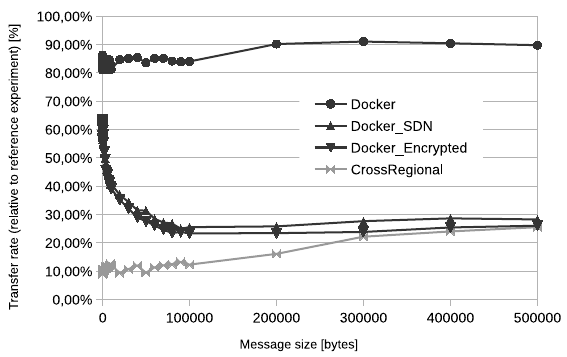
\includegraphics[width=0.5\textwidth]{performance}
\end{figure}

\par Deci deși containerele sunt văzute ca având un impact mic asupra performanței, nu este întotdeauna cazul. Acestea oferă totuși o mai mare flexibilitate în cadrul sistemlor bazate pe microservicii, de aceea au devenit din ce în ce mai folosite în ultima perioadă.\citep{kratzke2017microservices}

\clearpage

\section{Evoluție} Arhitectura este cea care permite unui sistem să evolueze și oferă un nivel de serviciu de-a lungul ciclului de viață. În ingineria software, arhitectura oferă o punte între funcționalitățile sistemului și cerințele de calitate pe care sistemul trebuie să le atingă. De-a lungul ultimelor decenii, arhitectura software a fost studiată intens și multiple feluri de a compune un sistem software au fost create, până să fie dezvoltată arhitectura bazată pe microservicii.\par Probleme asociate cu dezvoltarea de sisteme mari software a apărut pentru prima dată în jurul anilor 1960. Anii 1970 au însemnat un salt mare în interes pentru comunitatea de cercetători în domeniul proiectării acestor sisteme. În anii 1980, procesul de proiectare a fost integrat complet în cadrul procesului de dezvoltare a sistemelor software.\par
Prima referință a conceptului de arhitectură software a apărut pentru prima dat în anii 1980, dar prima definiție solidă a fost stabilită abia în anul 1992 de lucrarea \citep{perry1992foundations}. Popularitatea crescândă a paradigmei de programare orientată pe obiect a adus contribuții la dezvoltarea domeniului arhitecturii software, în anii 1990 în mod special.\par
Atenția oferită separării intereselor în cadrul unui sistem software a dus recent la așa numita inginerie software bazată pe componente, care a oferit un control mai bun asupra proiectării, implementării și evoluției sistemelor software.\par
Sistemelor orientate pe servicii sunt o paradigmă folosită pentru dezvoltarea de sisteme distribuite care își are originile în programarea orientată pe obiect și pe componente. Aceasta a fost introdusă pentru a valorifica complexitatea sistemelor distribuite și pentru a integra diferite aplicații software. Beneficiile orientării către servicii sunt:
\begin{itemize}
  \item dinamismul
  \item modularitatea și refolosirea
  \item dezvoltarea distribuită
  \item integrarea sistemelor heterogene și moștenite
\end{itemize}\par
Prima generație de arhitecturi de sisteme orientate pe servicii (SOA) a definit cerințe descurajante pentru servicii (descoperire și contracte între servicii), care au prevenit adoptarea acestui model. Microserviciile reprezintă a doua iterație a acestor concepte de arhitecturi orientate pe servicii. Scopul aceste iterații este de a îndepărta nivelele de complexitate inutile pentru a se pune accentul pe dezvoltarea de servicii simple care implementează eficient o funcționalitate.\par
Termenul de microservicii a fost introdus pentru prima dată în 2011 la un workshop de arhitectură software. Dar abordarea definită de acest termen era deja folosită, de exemplu în cadrul companiei Netflix, sub numele de \textit{Fine Grained SOA}\par
Microserviciile sunt un trend nou în arhitectura software și oferă caracteristici distinctive facă de predecesorul SOA: mărimea unui serviciu este mică, contextul fiecăruia bine definit, iar funcționarea este independentă.\par Caracteristicile cheie ale unui sistem bazat pe microservicii sunt:
\begin{itemize}
  \item flexibilitatea
  \item modularitatea
  \item evoluția
\end{itemize}\par
Microserviciile au câștigat popularitate recent și încă există o lipsă de consens cu privire la ce anume reprezintă acestea de fapt. M. Fowler și J. Lewis oferă un punct de pornire prin definirea principalelor caracteristici, iar S. Newman oferă soluții și practici cu privire la această arhitecură.\citep{newman2015building}\par
Dar acest sistem arhitectural este atât de nou încât putem spune că explorarea lui abia a început. Principala tărie a acestei abordări arhitecturale vine din distribuirea universală, chiar și a componentelor interne software, ca servicii autonome, care crează sisteme decuplate. În același timp, tot din acest aspect al distribuirii, rezultă și cea mai mare slăbiciune: programarea sistemelor distribuite este în esență mai grea decât programarea unor sisteme monolitice. Alte câteva exemple de posibile slăbiciuni ale acestei abordări vin din modul în care se pot gestiona schimbările asupra unui serviciu fără a afecta celelalte servicii cu care acesta comunică sau cum pot fi prevenite atacurile care încearcă să exploateze comunicațiile prin rețea. De asemeanea, prevenirea erorilor de programare este mai grea în cadrul acestor sisteme.

\clearpage

\section{Concluzii}
Arhitectura bazată pe microservicii este un stil arhitectural care a câștigat popularitate în ultimii ani atât în mediul academic, cât și lumea industriei software. În particular, adoptarea microserviciilor este chestiune sensibilă pentru un număr de companii implicate în refactorizarea majoră a sistemelor back-end. În ciuda faptului că este prezentat ca un concept revoluționar, este mai mult unul evoluționar. Fiind un concept recent, nu este dezvoltată încă o literatură cuprinzătoare în jurul lui. Rămâne de văzut dacă acest stil se va dovedi unul de succes, multe companii adoptând acest șablon pentru sistemele proprii, rezultatul acestei adopții putând fi observat de-a lungul anilor, prin performanța și valoarea pe care o aduc, și prin ușurința cu care pot fi modificare și evoluate.

\clearpage

%----------------------------------------------------------------------------------------
%	BIBLIOGRAPHY
%----------------------------------------------------------------------------------------

\printbibliography[title={Bibliography}] % Print the bibliography, section title in curly brackets

%----------------------------------------------------------------------------------------

\end{document}
